\documentclass{article}
\usepackage{tikz}
\usepackage{pgfplots}
\pgfplotsset{compat=1.18}
\usetikzlibrary{arrows.meta,positioning}
\begin{document}
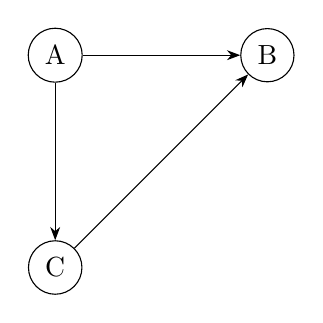
\begin{tikzpicture}[node distance=2cm, every node/.style={draw, circle}]
  \node (a) {A};
  \node (b) [right=of a] {B};
  \node (c) [below=of a] {C};
  \draw[-{Stealth}] (a) -- (b);
  \draw[-{Stealth}] (a) -- (c);
  \draw[-{Stealth}] (c) -- (b);
\end{tikzpicture}

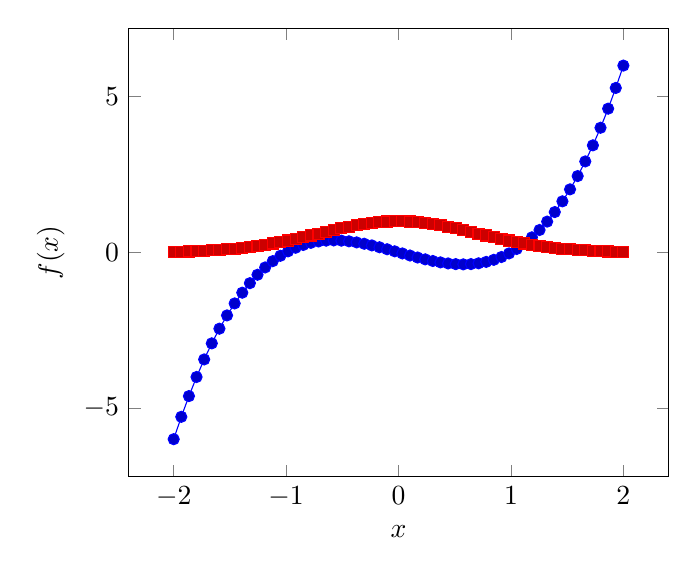
\begin{tikzpicture}
  \begin{axis}[xlabel=$x$, ylabel=$f(x)$, domain=-2:2, samples=60]
    \addplot {x^3 - x};
    \addplot {exp(-x^2)};
  \end{axis}
\end{tikzpicture}
\end{document}
